%!TEX root = ../main.tex
\setcounter{chapter}{7}
\setcounter{section}{3}
\section{Hardware Characteristics}
\vspace{-8pt} \hrule \hrule \hrule \hrule \hrule  \vspace{12pt}
\begin{itemize}
	\item Analog-to-Digital (A/D) Converter는 센서로 획득한 전압값을 컴퓨터에서 연산할 수 있는 digital값으로 변환해주는 장치
	\begin{itemize}
		\item Counting scheme 
		\item Successive-approximation technique 

	\end{itemize}
	\item Digital-to-Analog (D/A) Converter 컴퓨터로부터 만들어진 digital word를 전압값으로 변환해주는 장치, 일반적으로 A/D converter보다 싸다!
	\item 컴퓨터는 compensation $D_d(z)$를 프로그래밍하고, 계산하는 장치이다.
%
\newpage
%
	\item Analog Anti-Alias Prefilter는 아날로그 센서와 A/D converter 사이에 위치한다. 
	\begin{itemize}
		\item Aliasing은 아날로그 신호의 Maximum Frequency의 두배 이상의 Sampling Frequency를 사용하지 않은 경우, 아날로그 신호 주파수의 변형을 일으켜 디지털 신호로 변환 후에 다시 원래의 아날로그 신호를 복원하지 못하게 되는 현상을 뜻함.
		\begin{align*}
				y(t) = \sin(2 \pi \cdot 55t) +\sin(2\pi \cdot 120t) ~~~~~ \text{Maximum Frequency is 120 [Hz]}
		\end{align*}
		\begin{enumerate}
			\item 만일 Maximum Frequency의 2배보다 작은 Sampling Frequency $F_s$ = 200 \text{[Hz]}, $kT = k/200$ 라면,
				\begin{align*}
					y(kT) &=   \sin(2 \pi \cdot \frac{55}{200}  k) +\sin(2\pi \cdot \frac{120}{200}  k)\\
					      &=   \sin(2 \pi \cdot \frac{55}{200}  k) +\sin(\frac{6\pi}{5}  k)\\
					      &=   \sin(2 \pi \cdot \frac{55}{200}  k) +\sin((\pi + \frac{1}{5}\pi) k)\\
					      &=   \sin(2 \pi \cdot \frac{55}{200}  k) +\sin((2\pi - \frac{4}{5}\pi) k)\\
					      &=   \sin(2 \pi \cdot \frac{55}{200}  k) +\sin((- \frac{4}{5}\pi) k) ~~~~~~(\because \sin(\alpha) = \sin(2\pi k+ \alpha) )\\
					y_r(t)&=    \sin(2 \pi \cdot 55t) +\sin(-2\pi \cdot 80t)\\
				\end{align*}
				기존 아날로그 신호의 120[Hz]는 Aliasing으로 인해 Nyquist Frequency 기준으로 대칭되어, 80[Hz]성분의 주파수로 변경됨. 
				\newpage		
		\end{enumerate}

		\item 결국 Aliasing이 발생하지 않도록 하려면 Sampling Frequency 보다 큰 주파수에 대해서는 모두 Lowpass Filter 처리해서 제거한 후에 샘플링을 진행해야 하며 이러한 방식의 LPF를 Anti-Alias Prefilter라는 이름으로 사용한다.
		\begin{align*}
				y(t) = \sin(2 \pi \cdot 55t) +\cancel{\sin(2\pi \cdot 120t)} ~~~~~ \text{Anti-Aliasing over $2 F_s$}
		\end{align*}	
		\begin{align*}
			y(kT) &=   \sin(2 \pi \cdot \frac{55}{200}  k) \\
			y_r(t)&=    \sin(2 \pi \cdot 55t) \\
		\end{align*}

		\item In a continuous system, noise components with a frequency much higher than the control-system bandwidth normally have a small effect because the system will not respond at the high frequency. 
		
		\item However, in a \emph{digital system}, the frequency of the noise can be \emph{aliased down}  to the vincinity of the system bandwidth so the closed-loop system would respond to the noise.
		\item The solution to prevent aliasing is to place an analog prefilter before the sampler. In many cases, a simple first-order low-pass filter will do - that is - 
		\begin{align*}
			H_p(s) = \frac{a}{s+a}
		\end{align*}
		where the \emph{breakpoint} $a$ is selected to be lower than Nyquist rate $\omega_s/2$ so that any noise present with frequencies greater than Nyquist rate is attenuated by the prefilter. 
		\item If $\omega_s$ is chosen to be $25 \times \omega_{bd}$, the anti-aliasing filter breakpoint $a$ should be selected lower than $\omega_s/2$, so that 
		\begin{align*}
			a = 10 \times \omega_{bd} ~~~~\leftarrow~~~~ \omega_s = 25 \times \omega_{bd} 
		\end{align*}
		would be a reasonable choice. 
	\end{itemize}
\end{itemize}
%
%
\newpage
%
\section{Sample-Rate Selection}
%
\begin{itemize}
	\item The inherent approximation for the discrete TF may give rise to \emph{decreased performance} or even \emph{system instability} as the sample rate is lowered. This can lead the designer to conclude that a faster sample rate is required. 
	\item The \emph{sampling theorem} states that in order to reconstruct an unknown, band-limited, continuous signal from samples of that signal, we must \emph{sample at least twice as fast as the highest frequency contained in the signal}. $\omega_s = 2 \omega_{bd}$  
	\item In the $z$-plane, the highest frequency that can be represented by a discrete system is $\omega_s/2$. 
	\item For a very high frequency noise, it would be foolish to sample fast enough to attenuate the disturbance without the use of a prefilter. 
\end{itemize}
%
%
\newpage
%
\section{Discrete Design} 
%
\begin{itemize}
	\item This plant model can be used as part of a discrete model of the feedback system including the compensation $D_d(z)$. 
	\item Analysis and design using this discrete model is called \emph{discrete design} or alternatively, \emph{direct digital design}. 
	\item For a plant described by $G(s)$ and preceeded by a ZOH, the discrete TF was essentially given by 
	\begin{align*}
		G(z) = (1-z^{-1}) \mathcal{Z} \left\{ \frac{G(s)}{s} \right\}
	\end{align*}
	\begin{figure}[h]
		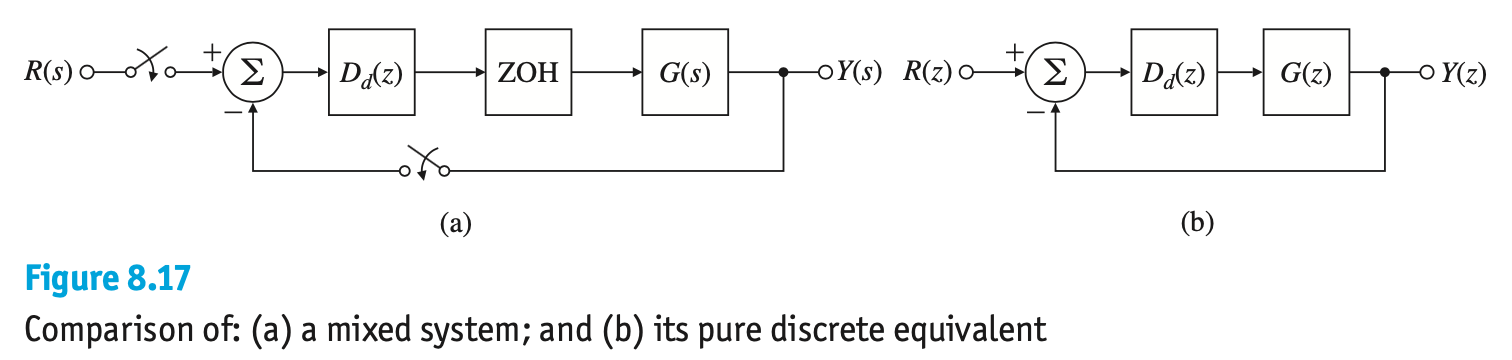
\includegraphics[width=12cm]{./FIG_Franklin/fig8-17.png}
	\end{figure}
	\item The closed-loop poles or the roots of the discrete characteristic equation
	\begin{align*}
		1+ D_d(z) G(z) = 0 
	\end{align*}
	\item The root-locus techniques used in continuous systems to find roots of a polynomial in $s$ apply equally well and without modification to the polynoimal in $z$.
	\item The interpretation of the results is that the stability boundary is now the unit circle instead of the imaginary axis. 
%
\end{itemize}
%

(Example 8.4)  When $G(s) = \frac{a}{s+a}$ and $D_d(z) = K$, draw the root locus with respect to $K$? 

(Answer) 
\begin{align*}
	G(z) &= (1-z^{-1}) \mathcal{Z} \left\{ \frac{a}{s(s+a)} \right\} = (1-z^{-1}) \mathcal{Z} \left\{ \frac{1}{s}  - \frac{1}{s+a} \right\} \\
	&= (1-z^{-1}) \left( \frac{1}{1-z^{-1}} - \frac{1}{1-e^{-aT}z^{-1}} \right)  \\
	&= \frac{(1-e^{-aT})z^{-1}}{1-e^{-aT}z^{-1}} \\
	&= \frac{(1-\alpha)z^{-1}}{1-\alpha z^{-1}} ~~~~~~~\mbox{where}~~ \alpha = e^{-aT}
\end{align*}
The discrete characteristic equation becomes
\begin{align*}
	1+ D_d(z) G(z) = 1 + K\frac{(1-\alpha)z^{-1}}{1-\alpha z^{-1}}= 0 
\end{align*}

\begin{figure}[h]
	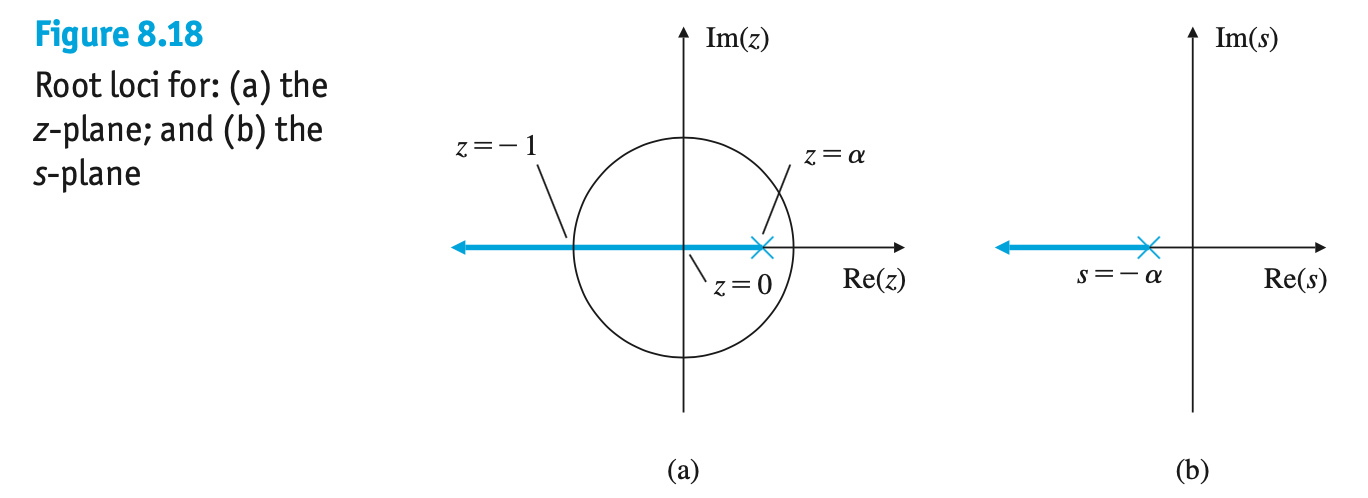
\includegraphics[width=12cm]{./FIG_Franklin/fig8-18.png}
\end{figure}

In the continuous case, the system remains stable for all values of $K$. 
In the discrete case, the system becomes oscillatory with decreasing damping ratio as $z$ goes from 0 to -1 and eventually becomes unstable. This instability is due to the lagging effect of the ZOH. 

%
\newpage
%
Feedback properties 
\begin{itemize}
	\item Proportional 
	\begin{align*}
		u(k) = Ke(k) ~~~~\leftrightarrow~~~~ D_d(z) = K 
	\end{align*}
	\item Derivative 
	\begin{align*}
		u(k) = K T_D [e(k) - e(k-1)] ~~~~~\leftrightarrow~~~~ D_d(z) = KT_D (1-z^{-1})
	\end{align*}
	\item Integral 
	\begin{align*}
		u(k) = u(k-1) + \frac{K}{T_I} e(k) ~~~~~\leftrightarrow~~~~ D_d(z) = \frac{K}{T_I} \left( \frac{1}{1-z^{-1}} \right) 
	\end{align*}
	\item Lead 
	\begin{align*}
		u(k) = \beta u(k-1) + K [e(k) - \alpha e(k-1)] ~~~~~\leftrightarrow~~~~ D_d(z) = K \frac{1- \alpha z^{-1}}{1-\beta z^{-1}} 
	\end{align*}
\end{itemize}
%
%
\newpage
%
%
\newpage
%
(Example 8.5)  Design a digital controller to have a closed-loop natural frequency $\omega_n = 0.3$ and a damping ratio $\zeta = 0.7$ using discrete design

(Answer) 
\begin{align*}
	G(s) = \frac{1}{s^2}   ~~~~~\rightarrow~~~~~~ G(z) = (1-z^{-1}) \mathcal{Z} \left\{ \frac{1}{s^3} \right\} = \frac{T^2}{2} \frac{z^{-1}(1+z^{-1})}{(1-z^{-1})^2}
\end{align*}
which, with $T=1$, becomes
\begin{align*}
	G(z) = \frac{1}{2} \frac{z^{-1}(1+z^{-1})}{(1-z^{-1})^2}
\end{align*}
Let us assume that the PD compensator is used
\begin{align*}
	D_d(z) = K (1- \alpha z^{-1})
\end{align*}
The desired pole locations of $\omega_n = 0.3$ and $\zeta = 0.7$ become $z=0.78 \pm 0.18j$ 
\begin{align*}
	1 + D_d(z) G(z) = 1 + K\frac{1}{2} \frac{z^{-1}(1+z^{-1})(1- \alpha z^{-1})}{(1-z^{-1})^2} =0 
\end{align*}
Now we have 
\begin{align*}
	\alpha = 0.85 ~~~~~~~~~~K = 0.374
\end{align*}
and 
\begin{align*}
	D_d(z) = 0.374 (1- 0.85 z^{-1})
\end{align*}
The difference equation becomes
\begin{align*}
	u(k) =  0.374 [e(k) - 0.85 e(k-1)] 
\end{align*}

(8장 숙제) 8장 연습문제에서 기말고사에 출제될 만한 문제 3개를 선택하여 풀어 제출하라? (마감 기말고사 전) 
% 
\newpage
